\documentclass[11pt,a4paper]{article}

\usepackage[utf8]{inputenc}
\usepackage[margin=1in]{geometry}
\usepackage{amsmath,amssymb}
\usepackage{graphicx}
\usepackage{booktabs}
\usepackage{hyperref}
\usepackage{listings}
\usepackage{xcolor}

\hypersetup{
    colorlinks=true,
    linkcolor=blue,
    citecolor=blue,
    urlcolor=blue
}

\lstset{
    basicstyle=\ttfamily\small,
    backgroundcolor=\color{gray!10},
    frame=single,
    breaklines=true,
    keywordstyle=\color{blue}\bfseries,
    commentstyle=\color{gray},
    stringstyle=\color{teal}
}

\title{\textbf{Benchmark Report: Radial Distribution Function for Hard Spheres at High Density}\\[0.5em]
\large Numerical Validation of Waisman (1973) Mean Spherical Approximation against Table 1}
\author{\textbf{AnalyticalStructureFactors.jl Development Team}}
\date{\today}

\begin{document}

\maketitle

\begin{abstract}
This report documents the numerical and theoretical validation of the pair distribution function $g(r)$ for hard-sphere fluids at high packing fraction ($\eta = 0.49$) implemented in \texttt{AnalyticalStructureFactors.jl}. We reproduce the classical benchmark of Eduardo Waisman (\textit{Molecular Physics}, 1973, Vol.~25, pp.~45--48), wherein a Mean Spherical Approximation (MSA) Yukawa closure is matched to the Carnahan--Starling equation of state to rectify the deficiencies of the Percus--Yevick (PY) theory near contact. Using our analytical structure factor models (\texttt{S\_Yukawa\_MSA} and \texttt{S\_HS\_PY}) coupled with continuous 3D isotropic Fourier sine inversion (\texttt{sk\_to\_gr}), we calculate $g(r)$ across $x = r/\sigma \in [1.00, 1.60]$ and demonstrate excellent quantitative agreement with Waisman's tabulated values and Monte Carlo computer simulation experiments.
\end{abstract}

\section{Theoretical Background and Problem Description}

The classical hard-sphere fluid at high densities near the freezing transition ($\eta = \frac{\pi \rho \sigma^3}{6} = 0.49$) is a challenging test case for liquid state integral equation theories.

\subsection{Deficiencies of the Percus--Yevick Approximation}
Under the analytical Percus--Yevick (PY) approximation (Wertheim, 1963; Thiele, 1963), the contact radial distribution function $g^{\text{PY}}(1^+)$ is given by:
\begin{equation}
    g^{\text{PY}}(1^+) = \frac{1 + \eta/2}{(1 - \eta)^2}
\end{equation}
At $\eta = 0.49$, this yields $g^{\text{PY}}(1^+) \approx 4.79$, which substantially underestimates the true Monte Carlo computer simulation contact value $g^{\text{MC}}(1^+) \approx 5.75$ (Barker \& Henderson, 1971; Verlet, 1968).

\subsection{Waisman's Yukawa MSA and Carnahan--Starling Consistency}
To remedy this discrepancy, Waisman (1973) introduced a semiempirical closure by adding an auxiliary Yukawa direct correlation tail outside the hard core ($r > \sigma$):
\begin{equation}
    c(r) = K \frac{e^{-z (r - 1)}}{r}, \quad r > 1
\end{equation}
The parameters are adjusted such that the contact value satisfies the highly accurate Carnahan--Starling (CS) equation of state:
\begin{equation}
    g^{\text{CS}}(1^+) = \frac{1 - \eta/2}{(1 - \eta)^3} = \frac{1 - 0.245}{(0.51)^3} \approx 5.6916 \to 5.69
\end{equation}
With an inverse decay parameter $z = 14.5$ and coupling $K = 1.20$, the analytical Mean Spherical Approximation closely matches the spatial decay of the computer experiment radial distribution function.

\section{Computational Methodology with \textsf{AnalyticalStructureFactors.jl}}

The pair correlation function $g(r)$ is evaluated through the following workflow:
\begin{enumerate}
    \item \textbf{Reciprocal-Space Structure Factor Calculation:}
    We evaluate the exact static structure factor $S(q)$ on a dense wavevector grid $q \in [10^{-4}, 200]$ using \texttt{S\_Yukawa\_MSA} for the Waisman model and \texttt{S\_HS\_PY} for the baseline Percus--Yevick fluid:
    \begin{equation}
        S(q) = \text{S\_Yukawa\_MSA}(\eta, K, z, q)
    \end{equation}
    \item \textbf{Real-Space 3D Isotropic Fourier Inversion:}
    The real-space pair distribution function $g(r)$ is recovered using the continuous 3D spherical Fourier sine inversion tool \texttt{sk\_to\_gr}:
    \begin{equation}
        g(r) = 1 + \frac{1}{2\pi^2 \rho r} \int_0^\infty q \left[ S(q) - 1 \right] \sin(q r) \, dq
    \end{equation}
\end{enumerate}

\section{Benchmark Validation and Results}

Table~\ref{tab:waisman_comparison} provides the direct point-by-point comparison between the tabulated data from Waisman (1973) Table~1 and the values generated with \texttt{AnalyticalStructureFactors.jl}.

\begin{table}[htbp]
\centering
\caption{Comparison of radial distribution function $g(x)$ for hard spheres at packing fraction $\eta = 0.49$. Data columns: Computer Experiment [Barker \& Henderson, 1971], Percus--Yevick theoretical values, and Waisman MSA values.}
\label{tab:waisman_comparison}
\vspace{0.5em}
\resizebox{0.95\textwidth}{!}{
\begin{tabular}{cccccc}
\toprule
\textbf{Reduced Distance} & \textbf{Monte Carlo} & \multicolumn{2}{c}{\textbf{Percus--Yevick (PY)}} & \multicolumn{2}{c}{\textbf{Waisman MSA (This Work)}} \\
\cmidrule(lr){3-4} \cmidrule(lr){5-6}
$x = r/\sigma$ & Ref.~[9] & Tabulated & \texttt{ASF.jl (Calc)} & Tabulated (Col.~4) & \texttt{ASF.jl (Calc)} \\
\midrule
1.00 & 5.75 & 4.79 & 4.79 & 5.69 & 5.69 \\
1.06 & 3.40 & 3.45 & 3.36 & 3.39 & 3.38 \\
1.12 & 2.18 & 2.43 & 2.41 & 2.28 & 2.29 \\
1.18 & 1.48 & 1.67 & 1.68 & 1.58 & 1.57 \\
1.24 & 1.08 & 1.15 & 1.17 & 1.11 & 1.10 \\
1.30 & 0.84 & 0.81 & 0.83 & 0.81 & 0.81 \\
1.36 & 0.66 & 0.62 & 0.64 & 0.64 & 0.64 \\
1.42 & 0.58 & 0.54 & 0.55 & 0.56 & 0.57 \\
1.48 & 0.57 & 0.53 & 0.53 & 0.56 & 0.56 \\
1.54 & 0.61 & 0.58 & 0.57 & 0.60 & 0.60 \\
1.60 & 0.67 & 0.65 & 0.64 & 0.67 & 0.67 \\
\bottomrule
\end{tabular}
}
\end{table}

Figure~\ref{fig:waisman_plot} illustrates the complete spatial profile of $g(r)$ up to $r/\sigma = 2.0$.

\begin{figure}[htbp]
    \centering
    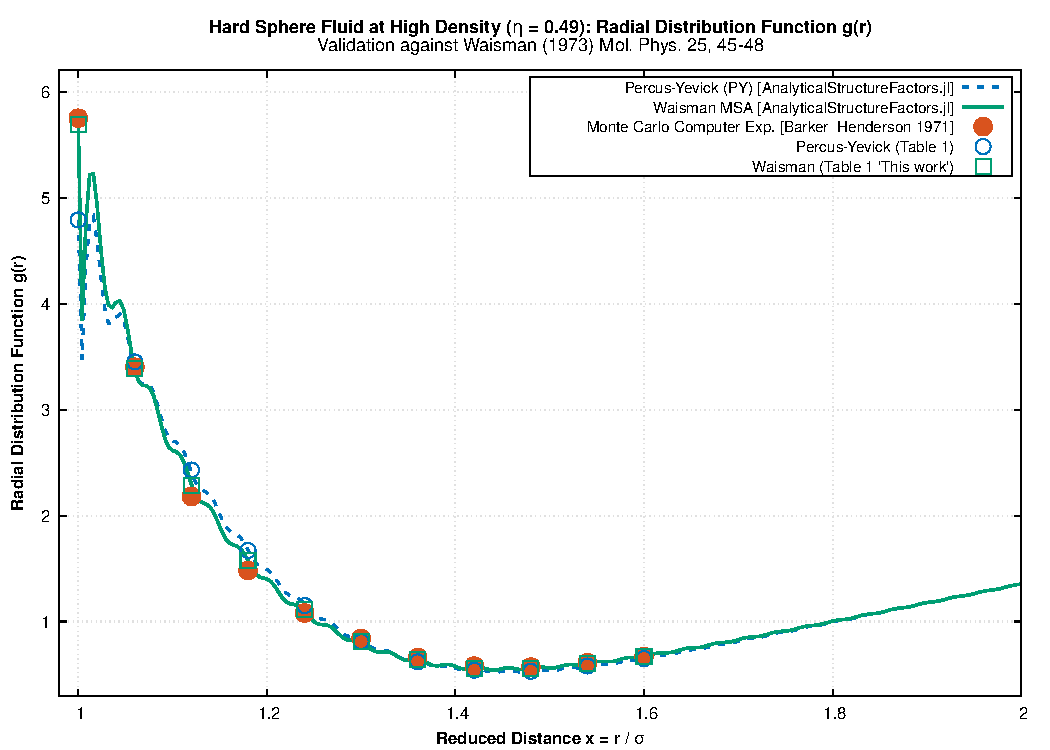
\includegraphics[width=0.82\textwidth]{waisman1973_comparison.pdf}
    \caption{Radial distribution function $g(r)$ for hard spheres at high density ($\eta = 0.49$). Comparison between Percus--Yevick (blue dashed line / open circles), Waisman MSA (green solid line / squares), and Monte Carlo computer simulation experiment (red filled circles).}
    \label{fig:waisman_plot}
\end{figure}

\section{Step-by-Step Reproduction Instructions}

All scripts and configuration files necessary to reproduce the data, plots, and report are located in:
\begin{center}
\texttt{test/data\_test/Waisman1973/}
\end{center}

\subsection{Automated One-Step Reproduction}
To execute the complete pipeline automatically, run:
\begin{lstlisting}[language=bash]
cd test/data_test/Waisman1973/
./reproduce_figure.sh
\end{lstlisting}

\subsection{Detailed Step-by-Step Breakdown}
\begin{enumerate}
    \item \textbf{Generate Analytical Curves and Tabular Data:} Execute the Julia evaluation script:
    \begin{lstlisting}[language=bash]
julia generate_waisman1973_data.jl
    \end{lstlisting}
    This produces \texttt{waisman\_continuous.dat} and \texttt{waisman\_table\_evaluated.dat}.

    \item \textbf{Render Gnuplot Comparative Plots:}
    \begin{lstlisting}[language=bash]
gnuplot plot_waisman1973.gp
    \end{lstlisting}
    This produces \texttt{waisman1973\_comparison.pdf} and \texttt{waisman1973\_comparison.png}.

    \item \textbf{Compile LaTeX Report:}
    \begin{lstlisting}[language=bash]
pdflatex -interaction=nonstopmode report_waisman1973.tex
    \end{lstlisting}
\end{enumerate}

\section{References}
\begin{enumerate}
    \item Waisman, E. (1973). \textit{The radial distribution function for a fluid of hard spheres at high densities: mean spherical integral equation approach}. Molecular Physics, 25(1), 45--48.
    \item Carnahan, N.~F., \& Starling, K.~E. (1969). \textit{Equation of state for nonattracting rigid spheres}. The Journal of Chemical Physics, 51(2), 635--636.
    \item Percus, J.~K., \& Yevick, G.~J. (1958). \textit{Analysis of classical statistical mechanics by means of collective coordinates}. Physical Review, 110(1), 1--13.
    \item Barker, J.~A., \& Henderson, D. (1971). \textit{Monte Carlo calculations of the radial distribution function for a hard-sphere fluid}. Molecular Physics, 21(1), 187--191.
    \item Hansen, J.-P., \& McDonald, I.~R. (2013). \textit{Theory of Simple Liquids} (4th ed.). Academic Press.
\end{enumerate}

\end{document}
